\subsection{Pantalla: Gestión de Proyectos}
\subsubsection{Objetivo}
	El mapa de navegación se muestra en la Figura~\ref{fig:mapaNavegacionCUC1}.

   \begin{figure}[hbpt!]
 		\centering
 			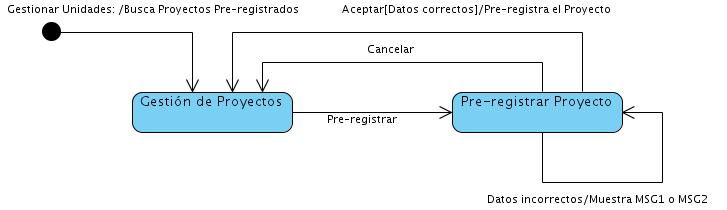
\includegraphics[width=0.8\textwidth]{images/CUC1/mapaNavegacion.jpg}
 		\caption{Mapa de navegacion para el CU C1 Gestion de Niveles.}
		\label{fig:mapaNavegacionCUC1}
 	\end{figure}

\subsubsection{Objetivo}
Mostrar la información correspondiente a los Proyectos Pre-registrados por el Coordinador que inicio sesión, con el fin de consultar el estado de cada Proyecto y la posibilidad de agregar uno nuevo, ver Figura~\ref{IUGestProyectos}. Viene de Menú Gestión de Catálogos.

\IUfig[0.7]{CUC1/GestionProyectos.png}{IUGestProyectos}{Gestión de Proyectos.}

\subsubsection{Salidas}
En esta pantalla se muestra la lista de Proyectos Pre-registrados. Los registros estan ordenados por nombre en una tabla.

\subsubsection{Comandos}
\begin{itemize}
 \item \IUbutton{
\includegraphics[scale=0.1]{images/icons/agregar.png}}:Esta opción permite Pre-registrar un nuevo Proyecto, al oprimirlo se mostrará la pantalla\IUref{IUPreregistrarProyecto}{Preregistrar Proyecto}Si el Proyecto se Pre-registra correctamente, este aparecerá en la tabla.
\end{itemize}